\section{Workflow}
\label{sec:wokflow}

A typical workflow of charge transport simulations is depicted in \fig{workflow}. The first step is the simulation of an \slink{morphology}{atomistic morphology}, which is then partitioned on \slink{segments}{hopping sites}. The coordinates of the hopping sites are used to construct a list of pairs of molecules, or \slink{neighborlist}{neighbor list}. 

\begin{figure}[h]
   \label{fig:workflow}
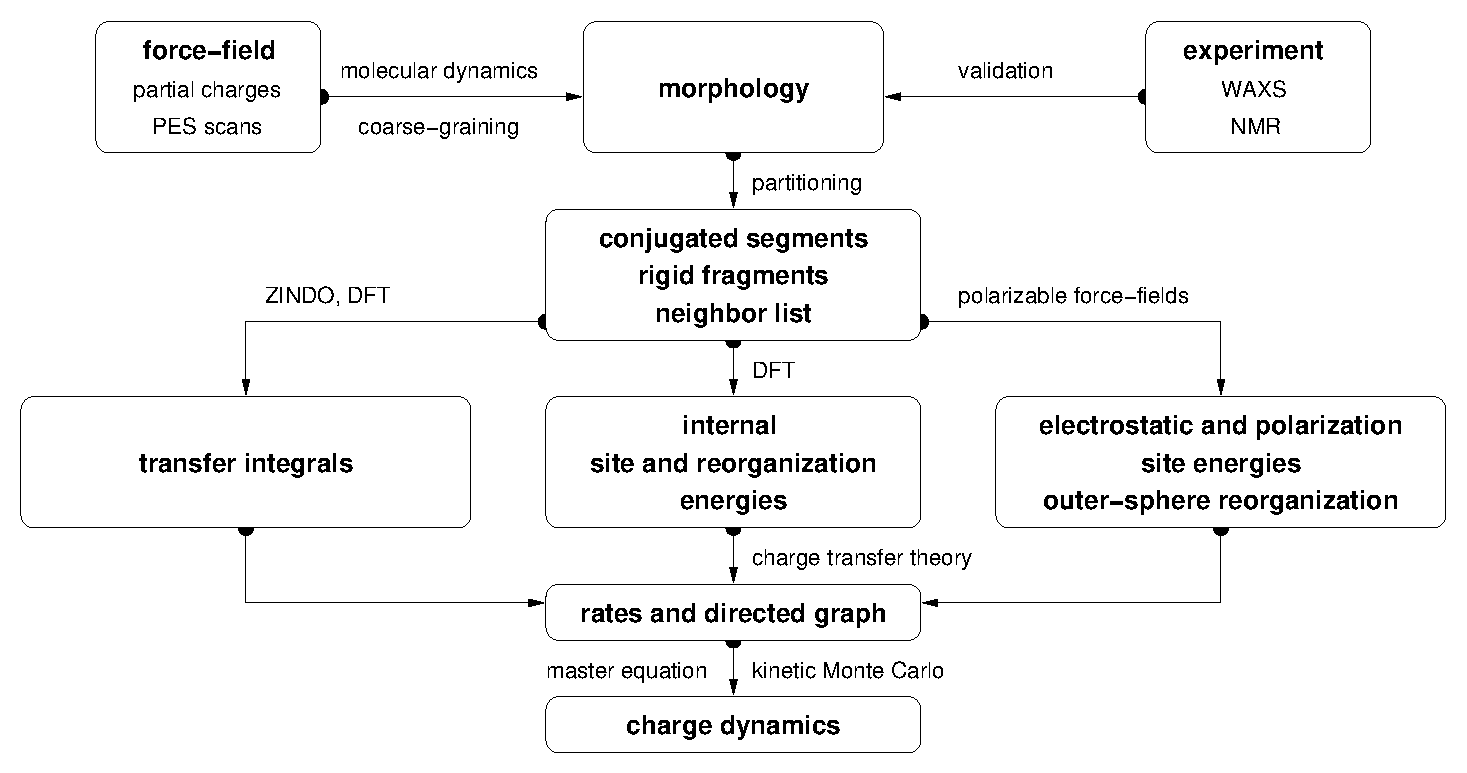
\includegraphics[width=\textwidth]{fig/workflow}
 \caption{%
   Workflow for microscopic simulations of charge transport.  %
}
\end{figure}

For each pair an \slink{transfer_integrals}{electronic coupling element}, a \slink{reorganization}{reorganization energy}, a \slink{site_energies}{driving force}, and eventually the \slink{rates}{hopping rate} are evaluated. The neighbor list and hopping rates define a directed graph. The corresponding master equation is solved using the \slink{kmc}{kinetic Monte Carlo} method, which allows to explicitly monitor the charge dynamics in the system as well as to calculate time or ensemble averages of occupation probabilities, charge fluxes, correlation functions, and field-dependent mobilities.

% 
% \begin{figure}[p]
% \includegraphics[width=\textwidth]{fig/workflow_practical/workflow_practical}
%  \caption{%
%    Workflow for microscopic simulations of charge transport including calls.  %
%    \label{fig:workflow}}
% \end{figure}



